\subsection{Estimation methods}
% 3 pages
Estimating the extent of tasks is always relevant, as it (obviously) gives an idea of how long each task probably will take to finish. Even though one does not always actively make these estimations on a small project/task, one does always have an idea of how long the individual tasks will take.

The knowledge is essential to plan a project, because the sum of all estimations sheds light on how long time the project probably will take, which in turn enables several different planning methods to be used, each providing a more-or-less optional route through the tasks.

The use of estimation methods allowed us to be precise and thorough in our estimations. Based on the knowledge acquired from the application of the methods, we could make more precise plans to help us overcome the derailed project.

In the following we will present the methods we have used to estimate our tasks for the project, and describe our thoughts on how we experienced the use of these.

\textbf{ [ TODO: Perhaps say something about, adding or removing items/functionality according to whether there is enough time or not ]}

\subsubsection{Planning Poker}
Multiple estimation methods exists, but for this part of the project, we have chosen to use Planning Poker, also know as SCRUM Poker, to estimate the remaining tasks at the backlog.

Planning Poker seemed like a good choice since we all have worked with SCRUM before, but not used Planning Poker. Now was a great opportunity to practice it.

We think that the fact that the players do not influence each other when estimating, while the game still facilitates shorts discussion, gives Planning Poker an advantage over traditional, discussion-only estimation.
That planning poker facilitates discussions is the reason for why we chose Planning Poker over the Delphi estimation method, which does not.

The discussion might not always be an advantage, though. It can easily become very time consuming. We chose a non-voting, but overruling, moderator to address this potential problem, and we believe it worked great proving an advantage multiple times.

\begin{figure}[t]
  \centering
  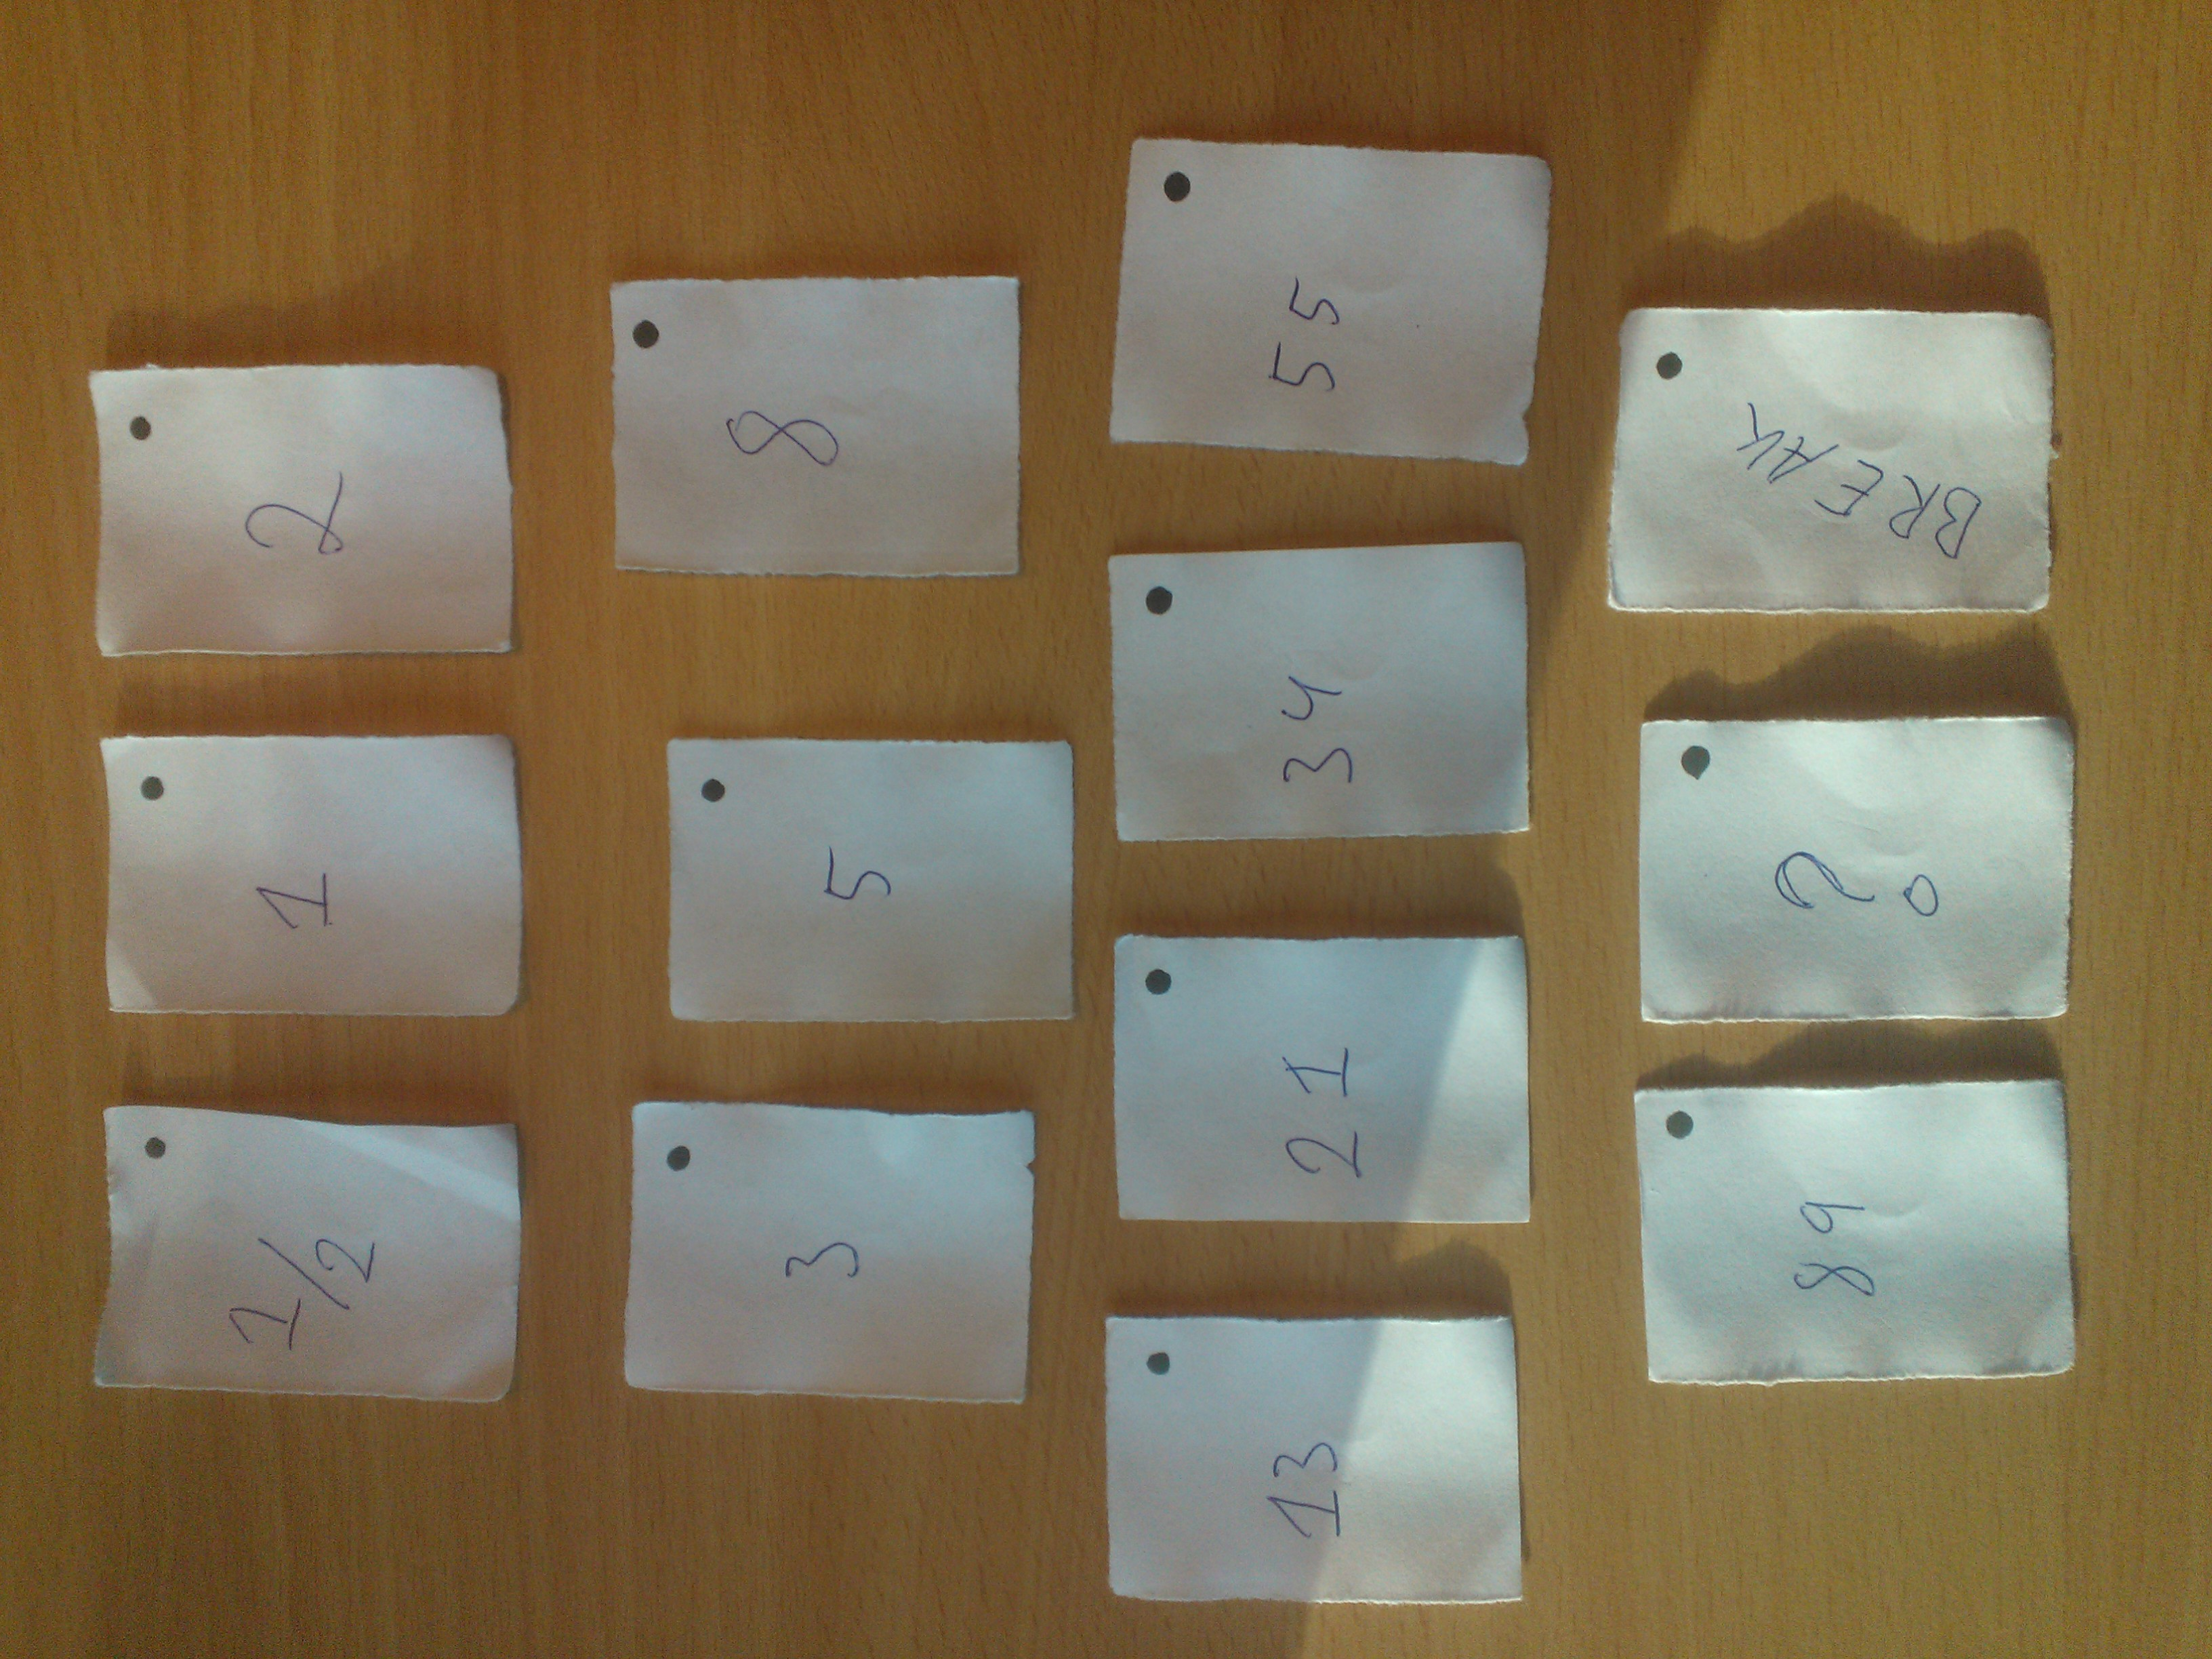
\includegraphics[width=\textwidth, angle=270]{illustrations/scrumPokerCards.jpg}
  \caption{SCRUM Poker cards}
  \label{fig:scrumPokerCards}
\end{figure}

For our game we made playing cards with the numbers 1/2, 1, 2, 3, 5, 8, 13, 21, 34, 55, 89, `?' and `break'. The numbers represented man hours and the question-mark represented that the `player' was unable to give a good estimate, while the "break" card represented that the player needed a short break from the game (see figure \ref{fig:scrumPokerCards}).

We found that using Planning Poker had several advantages over to what we previously had done. Compared to what we did in the first part of the project, we now got a real idea of how much time and effort we should put in each task - and in the rest of the project itself. Beside the work-related advantages we also found it way more motivating than other methods, and all members of the group was included in the process. Yet, the high numbers (55 and 89) was never used, as well as the `break' card. The `?' was only rarely used, and at last not considered a valid card by the team, due to the fact that when playing the card the player did not participate in the discussion. Also it introduced the risk of only one person having a real estimation vote for the task.

\subsubsection{CoCoMo estimation}
CoCoMo is an algorithmic software cost estimation method. With basic CoCoMo one can calculate time estimations depending on the size of the team and the experience of the team, combined with estimated Kilo Lines Of Code (KLOC) and factoring the programming language. It can also be used in other ways. Estimating the other variables, the remaining variable can be calculated, for example cost of project or team size required. One can add many more factors to the CoCoMo calculation: Complexity, reliability, hardware constraints, and more \cite[p. 147]{PM}.

We have chosen not to use the CoCoMo estimation. We do not have enough known variables to compute an estimate that is more accurate than using Planning Poker. Planning Poker also forces us to discuss each backlog item, as we disagree upon the estimation. The time spend discussing pulls the team together on the same page. 

\subsubsection{PERT estimation}
The last estimation method we have considered is the PERT estimation method. While most other methods only ends up with one estimation for each task, the PERT method uses three estimates, and then calculate it into one. The force of the PERT method lies in its three estimates \cite[p. 152]{PM}:

It is definitely a possibility to combine the Planning Poker method with the PERT method. Instead of each player only turning one card, each turns three cards: A optimistic estimate, a realistic estimate and a pessimistic estimate. So instead of having to agree on one estimate, the `players' would have to agree on all 3 estimates.

We did not use the PERT-method method (neither the "real" PERT, nor the PERT-Planning-Poker hybrid explained above), due to the fact that estimated it would take us much longer to make three estimates for each task, than only making one.